\documentclass[10pt, final, journal, letterpaper, twoside, twocolumn]{IEEEtran}
\usepackage[utf8]{inputenc}
\usepackage{indentfirst}
\usepackage{graphicx}
\usepackage{setspace}
\usepackage[numbers]{natbib}
\usepackage{layout}
\usepackage [english]{babel}
\usepackage [autostyle, english = american]{csquotes}
\MakeOuterQuote{"}
\usepackage[T1, hyphens]{url}
\urlstyle{same}
\usepackage[colorlinks=false, hidelinks, breaklinks]{hyperref}
\usepackage{breakurl}

\graphicspath{
	{.}
	{Sources/}
}

\begin{document}

\title{Assuring Software Quality Through the Use of Fuzzy Testing}
\author{\IEEEauthorblockN{David Jefts} \\
	\IEEEauthorblockA{SE625, Software Quality Assurance}}
\IEEEspecialpapernotice{Embry-Riddle Aeronautical University}
%\thanks{\LaTeX}
\markboth{Made with \LaTeX}{SE625}

\maketitle

%%%%%%
%I assume you will introduce the concept of Fuzzy testing, how it is used, where it is used, advantages disadvantages, etc. etc.   If this is correct, you are good to go.
%%%%%%

\begin{abstract}
	Ensuring that software works properly before public (or private) release is important because software bugs, or in-code errors, can cost the developing company a lot of money. Software bugs cause program faults, faults open up security vulnerabilities or cause program failures, and the maintenance and repair of software is 65-85\% of system development and deployment cost. Fuzzy Testing is a very easy-to-implement method of software penetration and quality assurance testing that is fully automated. This paper makes the case for a wider adoption of Fuzzy Testing in all software development projects, from private developers and end-users to multi-national corporations.
	%\textbf{\textit{THIS IS NOT MY ABSTRACT}} Software engineering researchers solve problems of several different kinds. To do so, they produce several different kinds of results, and they should develop appropriate evidence to validate these results. They often report their research in conference papers. I analyzed the abstracts of research papers submitted to ICSE 2002 in order to identify the types of research reported in the submitted and accepted papers, and I observed the program committee discussions about which papers to accept. This report presents the research paradigms of the papers, common concerns of the program committee, and statistics on success rates. This information should help researchers design better research projects and write papers that present their results to best advantage. 
	
	%This paper makes the case for TaaS—automated software testing as a cloud-based service. We present three kinds of TaaS: a “programmer’s sidekick” enabling developers to thoroughly and promptly test their code with minimal upfront resource investment; a “home edition” on-demand testing service for consumers to verify the software they are about to install on their PC or mobile device; and a public “certification service,” akin to Underwriters Labs, that independently assesses the reliability, safety, and security of software.
	%TaaS automatically tests software, without human involvement from the service user’s or provider’s side. This is unlike today’s “testing as a service” businesses, which employ humans to write tests. Our goal is to take recently proposed techniques for automated testing—even if usable only on toy programs—and make them practical by modifying them to harness the resources of compute clouds. Preliminary work suggests it is technically feasible to do so, and we find that TaaS is also compelling from a social and business point of view.
\end{abstract}

\begin{IEEEkeywords}
	Fuzzy Testing, Fuzz Testing, Fuzzing, Smart Fuzzing, Fuzzers, Software Quality Assurance, Quality Assurance, Software Vulnerabilities, Software Reliability, Testing, Automated Testing, Error Detection, Software Errors, Debugging, Computer Bugs, Computer Security, Testing, Product Testing, System Testing, Software Penetration Testing
\end{IEEEkeywords}

\section*{Nomenclature}
\addcontentsline{toc}{section}{Nomenclature}
\begin{IEEEdescription}[\IEEEusemathlabelsep\IEEEsetlabelwidth{$V_1,V_2,V_3$}]
\item[AI] Artificial Intelligence
\item[CPU] Computer Processing Unit
\item[CVE] Common Vulnerabilities and Exposures
\item[DoS] Denial of Service
\item[FC] Fuzzy Clustering
\item[FDA] United States Food and Drug Administration
\item[GA] Genetic Algorithm
\item[HTML] Hypertext Markup Language
\item[HTTP] Hypertext Transfer Protocol
\item[IE] Microsoft's Internet Explorer Web Browser
\item[IM] Instant Messaging
\item[OSS] Open Source Software
\item[POST] HTTP Request Method used by the World Wide Web
\item[RISC] Reduced Instruction Set Computer
\item[SAGE] Scalable, Automated, Guided Execution
\item[SSL] Secure Sockets Layer
\item[TLS] Transport Layer Security
\item[VPN] Virtual Private Network\\
\end{IEEEdescription}

\section{\label{sec:introduction}Introduction}
	%Introduction
	\IEEEPARstart{E}{nsuring} that software works properly before public (or private) release is important because software bugs, or in-code errors, can cost the developing company a lot of money. Software bugs cause program faults, faults open up security vulnerabilities or cause program failures, and the maintenance and repair of software is 65-85\% of system development and deployment cost \cite{slide-defect}. Naturally, the goal during software development is to limit these defects by testing the software before release. However, "software testing is a very labor intensive and costly task, [even though] many software testing techniques to automate the process of software testing have been [designed and] reported in the literature" \cite{fuzzy-logic}. One such technique is Fuzzy Testing, also called Fuzzing.
	
	%Why I chose this topic
	Fuzzy testing is an important topic to study because it offers a fully automated way to test software that is reliable. What is most interesting about it is that it incorporates many different fields from the software and computer fields: Software Development/Engineering is the main application of Fuzzy Testing, Software Quality Assurance is the entire goal of Fuzzy Testing, Artificial Intelligence and Machine Learning are being used to help optimize various fuzzy testing techniques, and Software Penetration and Security Testing also uses Fuzzy Testing to "verify security functionality" \cite{penetration}.
	
	%Goal of this paper
	This paper seeks to summarize much of the leading-edge research on fuzzy testing. It makes the case for a more proliferated use of fuzzy testing in the software industry and promotes additional research for better ways to optimize fuzzy testing. "Automated software testing, available to anyone and everyone at low cost, can transform the current development paradigm into one that involves more-thorough yet less-time-consuming testing" \cite{automation}. By promoting fuzzy testing as a whole, along with further development of fuzzy testing, automated software testing can be made more reliable and easier to access.
	
	%Organization
	The rest of this paper is organized as follows. The general types of software testing and their breakdowns are discussed in Section \ref{sec:software}. In Section \ref{sec:fuzz}, Fuzzy Testing and its real-world applications are presented. Section \ref{sec:industry} breaks down Fuzzy Testing and enumerates its various techniques and real-world applications. Section \ref{sec:bugs} details many of the popular applications and frameworks that use fuzzy testing, along with many public security vulnerabilities and threats that were found with fuzzy testing. This paper presents the argument for the adoption of Fuzzy Testing in Section \ref{sec:compare} along with comparisons to other methods of software quality assurance testing. All conclusions and future projects are discussed in Section \ref{sec:conclude}.

\pagebreak
\section{\label{sec:software}Software Testing}
	%White Box Testing
	There are two main 'sectors', or approaches, to software testing: white-box testing and black-box testing \cite{boxes}. White Box Testing, also called Structural Testing \cite{slide-testing}, is the testing of a system \textit{with} knowledge of the internal systems software. Testers in this paradigm "have access to the source code and are aware of the system architecture" \cite{boxes}. Generally, White Box testers analyze the source code of the software and develop test cases and identify specific code paths to achieve the most raw code coverage. They develop test cases with respect to executed statements, branches, paths, and so forth. "After initial testing, programmers frequently face the problem of finding additional test data to evaluate program elements not yet covered" \cite{assertion}. Determining the test data required to evaluate 100\% of the software is often very labor-intensive and expensive. Test generators in the White Box testing paradigm work to find program input(s) on which a selected portion of the software is executed. According to \cite{assertion}, there are currently three types of automatic generators for this: \textit{random} test generators, \textit{path-oriented} generators, and \textit{goal-oriented} generators. White Box testing generally finds more bugs and defects as compared to Black Box Testing. However it requires more time and money than Black Box Testing, since it often requires a direct analysis of the source code and tests must cover 100\% of the code.
	
	%Black Box Testing
	Black Box Testing, also called Functional Testing \cite{slide-testing}, is the testing of a system with no knowledge or direct access of the internal systems in the software. Testers in this paradigm "do not have access to the source code and are oblivious of the system architecture" \cite{boxes}, and select test data "based on the functional specification of the program (e.g., equivalence class partitioning, boundary-value analysis)" \cite{assertion}. Black Box testers just test the software through the provided user interface and analyzing inputs and outputs for correctness. Test generators working off of the Black Box paradigm create test cases and test data by "using a set of rules and procedures; the most popular methods include equivalence class partitioning, boundary value analysis, [and] cause-effect graphing" \cite{assertion}. "By their nature Black Box testing methods might not lead to the execution of all parts of the code. Therefore, this method may not uncover all faults in the program" \cite{fuzzy-logic}. 
	
	%Grey Box Testing
	Grey Box Testing is a combination of White Box and Black Box Testing, which aims to take advantage of each of the aforementioned testing paradigms while minimizing their drawbacks. It generally uses only a minimal knowledge of the program structure and behavior. It does not require access to the source code and analyzes the software from an external perspective. Generally the tester will know how the internal system components interact, such as the internal data structures and algorithms \cite{gray}, but will not have a full and detailed knowledge about the internal program functions and/or operation. It offers a clear distinction between "the developer and tester, thereby minimizing the risk of personnel conflicts" \cite{gray}. 
	
	%Assertion-Based Testing
	Assertion-Based testing is reportedly a largely effective software testing technique \cite{assertion}. It involves finding program inputs in which various assertions are violated. When these assertions are violated then there is a fault in the program \cite{assertion}. Each assertion specifies "a constraint that applies to some state of a computation" \cite{assertion}, for example making sure that a variable holds valid data. Some languages support this by default for example Java and Perl, while others have libraries that . According to \cite{fuzzy-logic} it is fairly easy to generate assertion tests; "creating boundary checks, division by zero, null pointers, and variable overflow/underflow" \cite{fuzzy-logic}. The problem with this method of software testing is that the implementation of large amounts of assertions can be costly and is often impractical for industrial-sized software. Additionally, finding program inputs that cover all assertions in the software can be difficult and time consuming. 
	
	%Fuzzy Testing
	Fuzzy Testing can fall under White Box, Black Box, or a combination of both depending on how aware the tester is of the program structure. Fuzzy Testing is the process of submitting "malformed, malicious, and random data to a system's entry points [or user interface] in an attempt to uncover faults" \cite{penetration}. "The tool then reports the faults to the tester for further analysis" \cite{penetration}. Fuzzing may also be described as "a security testing approach based on injecting invalid or random inputs into a program in order to obtain an unexpected behavior and identify errors and potential vulnerabilities" \cite{vulnerabilities}. This method is generally much cheaper and easier to utilize than the others since it is designed to be automated, but it suffers from many of the same drawbacks as Black Box testing- namely that it does not guarantee full code coverage and therefore cannot guarantee the software is bug free. 


\section{\label{sec:fuzz}Fuzzy Testing}
	%Fuzzy testing techniques
	\subsection{\label{sec:techniques}Techniques}
		Fuzzy Testing is a negative-testing technique, used to find software bugs, faults, and vulnerabilities \cite{textbook}. While Fuzzy Testing is generally performed entirely automatically, it is also possible to perform semi-automated or even completely manual fuzzing \cite{break-software}. Manual testing involves finding data fields and modifying them to see if they break. Semi-automatic uses small scripts that are run individually to test the software. This paper is focused on fully automatic fuzzy testers, that use a script or program to iterate over an extensive list of possible inputs until the program crashes or has a fault \cite{fuzzing}. These inputs can be generated completely from scratch (random), in a brute-force manner (sequential generation of all possible input combinations), or with data mutation (capturing valid input data and mutating it, either randomly or in a brute-force manner) \cite{clarke}. These random inputs can be generated in a variety of ways but some more efficient fuzzers use genetic algorithms to `intelligently' generate test data \cite{ga}. All fuzzers share a similar set of features \cite{clarke}:
		
		\begin{itemize}
			\item{data generation (creating data to be passed to the target);}
			\item{data transmission (getting the data to the target);}
			\item{target monitoring and logging (observing and recording the reaction of the target), and;}
			\item{automation (reducing, as much as possible, the amount of direct user-interaction required to carry out the testing regime).}
		\end{itemize}
	
	Fuzzy testing is similar to stress testing, which involves sending an excessive amount of bogus data to a software or digital service with the goal of making it crash, to determine its stability and ensure that it is stable under normal operating conditions or to determine the limits of its use.
		
	%Analyze potential applications and best-case uses for fuzzy testing
	\subsection{Applications}
		Currently, the most popular application of fuzzy testing is for exposing security vulnerabilities in software products, either by hackers or software developers \cite{microsoft-penetration}. This is because fuzzers are often built to generate large amounts of potentially corrupt data in a relatively short time, allowing one to test a plethora of different edge cases that the original programmer may not have accounted for. Fuzzers are generally fairly effective at finding regular software bugs in applications that have a user input. The mass-production of random data is useful in finding edge-cases, corner cases, and boundary cases. Edge cases are software states that are generally only observed at extreme operation parameters (e.g. a stereo speaker operating at or beyond its maximum volume). Corner cases occur outside of normal operating parameters, when multiple variables and/or conditions are at extreme, albeit valid, levels. Boundary cases are software instances where an input, variable, or condition is at or beyond its maximum limits.
		
		"Anyone who has access to an application can fuzz it. Access to the source code is not required" \cite{clarke}. It requires very little expertise to identify basic bugs, as compared to White Box testing and Assertion-Based testing. Additionally, implementation is fast due to a wide variety of fuzzing applications and can take only a few minutes in some cases. Developers can apply fuzzy testing for vulnerability discovery and resolution during the entirety of the software development life-cycle. "Software vendors such as Cisco, Microsoft, Juniper, AT\&T, and Symantec all employ fuzzing as a matter of course" \cite{clarke}. End-users, small- to medium-sized enterprises, and corporations can all take advantage of fuzzers to use as a software quality assurance tool. Virtual attackers and hackers may also use fuzzing to identify and inject malicious data or code into Internet software to gain unintended access and exploit on-line systems. 
	
	
\section{\label{sec:industry}Large-Scale and High-Profile Utilizations of Fuzzing}
	%Examples of use of fuzzy testing in industry
	\subsection{The Monkey}
		First developed around 1983, The Monkey was one of the first tools to utilize fuzzy testing \cite{textbook}. "The Monkey was a small desk accessory that used the journaling hooks to feed random events to the current application, so the Macintosh seemed to be operated by an incredibly fast, somewhat angry monkey, banging away at the mouse and keyboard, generating clicks and drags at random positions with wild abandon" \cite{monkey}.
		
	\subsection{PROTOS}
		Short for \textit{Security Testing of Protocol Implementations}, PROTOS was a project initiated in 1999 through a joint effort between the University of Oulu and VTT Electronics \cite{protos}. It was originally proposed by Marko Laakso who was inspired by the large number of security problems in software in the 1990's. PROTOS has been used to break a wide variety of software systems including: Cisco Routers running Cisco IOS 12.2T and 12.2 `X' trains, AdventNet Web NMS 2.3, IBM SecureWay V3.2.1 running under Solaris and Windows 2000, and Qualcomm Eudora WorldMail for Windows NT, version 2.
		
	\subsection{SMUDGE}
		The \textit{Software Mutilation Utility and Data Generation Engine} is a fuzzing framework written in python by nd@felincemenace. It only performs network protocol fuzzing \cite{fuzzing}, but was used to break: Sambar webserver 0.5 overflow in POST handling, DoS in Helix Servers up to version 9.0.2, and not-exploitable overflows in IE Web Browser.
	
	\subsection{U.S. Food and Drug Administration Medical Cybersecurity Laboratory}
		One popular use of fuzzy testing was by the FDA, it "adopted a generational fuzzer as the foundation of its newly created cybersecurity laboratory, in which medical devices will be tested with the aim of improving safety and reliability" \cite{fda}. In July of 2014 the FDA reported that the first tool its lab would use was Defensics, a fuzz testing platform created by Codenomicon \cite{codenomicon}.
		
	\subsection{ClusterFuzz}
		On April 26\textsuperscript{th}, 2012, Google announced their cloud-based fuzzing infrastructure for finding security-critical components for Google's Chromium and Chrome web browsers \cite{clusterfuzz}. According to \cite{clusterfuzz}, it is highly scalable, has accurate deduplication of crashes, minimizes test cases, supports blackbox fuzzing, and offers statistics and regression finding for analysis of fuzzer performance.
		
	\subsection{mangleme}
		mangleme is a fuzzer tool written in C by Michał Zalewski, also known by the user name \textit{Icamtuf}. It is an automated broken HTML generator and browser tester released in 2004. It was used to find major security problems in all of the major web browsers including: Mozilla/Firefox/Netscape, Konqueror, Safari, Internet Explorer, Lynx, Opera, and Links.
		
	\subsection{Project Springfield}
	Microsoft announced its own cloud-based bug detector based off of SAGE, called Project Springfield, in 2016 \cite{springfield}. It is "one of the most sophisticated tools [Microsoft] has for rooting out potential security vulnerabilities in software" \cite{springfield}. Its main goal is to save software developers from having to take the "costly effort" of releasing a patch reactively, after it has already been deployed to the general public. 
		
	\subsection{OSS-Fuzz - Continuous Fuzzing for Open Source Software}
		Released in December 2016, OSS-Fuzz is a fuzz testing tool developed by Google and was mainly used by them to test their Google Chrome web browser \cite{oss-fuzz}. At the time of writing, it supported the C and C++ programming languages and reportedly found "hundreds of security vulnerabilities and stability bugs" \cite{oss-fuzz}.
		

\section{\label{sec:bugs}Security Threats Discovered with Fuzzy Testing}
	\subsection{Heartbleed}
	Officially referred to as `CVE-2014-0160', the Heartbleed Bug is a security vulnerability in the OpenSSL cryptographic software library. It allows the stealing of information normally protected by the SSL/TLS encryption used to secure the internet \cite{heartbleed}. "SSL/TLS provides communication security and privacy over the Internet for applications such as web, email, instant messaging (IM), and some virtual private networks (VPNs)" \cite{heartbleed}. It reveals the memory of systems normally protected by SSL/TLS to anyone who wishes to see it, allowing malicious people to gather names and passwords, eavesdrop on communications, steal data directly from services and users, and impersonate services and users. In April 2015, Hanno B\"{o}ck revealed that this bug could have been easily discovered with a "reasonably simple fuzzing setup \dots [that] doesn't require any prior knowledge about specifics of the Heartbleed bug or the TLS Heartbeat extension" \cite{hanno}.
	
	\subsection{GOD MODE UNLOCKED - Hardware Backdoors}
		In July of 2018, Christopher Domas revealed a hardware backdoor, colloquially called the \textit{rosenbridge}, in x86 CPUs developed by VIA Technologies, Inc. \cite{GOD}. Domas' backdoor "offers ring 3 (userland) to ring 0 (kernel) privilege escalation, providing a well-hidden, devastating circumvention to the long-standing x86 ring privilege model, wherein untrusted code is effectively separated from the heart of the system" \cite{GOD}. Domas surmised that the VIA Technologies Inc., C3 family of x86 processors had a second \textit{deeply embedded core} that was a RISC processor tightly connected to the main processor core. In \cite{GOD}, Domas used a processor fuzzing tool called \textit{Sandsifter} to help identify the \textit{god mode bit} to the RISC core. He also used \textit{Sandsifter} to find the \textit{bridge instruction} used to send and execute commands on the main x86 processor.
	

\section{\label{sec:compare}A Fuzzy Testing Comparison}
	%Advantages and disadvantages of fuzzy testing
	\subsection{Test Data Generation}
		The three methods of test data generation listed in Section \ref{sec:techniques} each have their own advantages and disadvantages. Figure \ref{fig:testdata} depicts a tabular comparison of these test data generation methods.
		
		\subsubsection{\label{sec:random}Random Data}
			Often referred to as `blind-fuzzing', this approach is desirable because it requires very minimal effort to initiate testing, and assumptions do not restrict the scope of testing \cite{clarke}. However, random test generation does not guarantee the generation of the combination(s) required to cause a failure. 
			
		\subsubsection{Brute-Force Data}
			This method involves sequentially building every possible permutation of the input space. Like the random data generation, this method requires no knowledge of the target system, with the exception that the size of the input space should be known in order to limit the amount of data generated \cite{clarke}. Brute-Force test data generation falls apart when there is a large input space, as it is very inefficient and will require more storage and/or time in order to exhaust every possible input. "In order to brute force fuzz all values of a 32-bit integer, a total of 4,294,967,295 test instances would be required. Disregarding the time and space required to generate and store this test data, it would take 500 days to process each of the required test instances assuming it would take one hundredth of a second to process each one" \cite{clarke}.
			
		\subsubsection{Data Mutation}
			This method involves capturing valid software input data while the software is in use, then modifying and mutating the data (either random or brute-force). The data capture step is generally basic and fast and due to the similarity to valid input, the generated test data will have a much higher efficiency \cite{clarke}. This allows the mutation method to have the advantages of random and brute-force test data: minimal required effort and knowledge of the data, while avoiding all of the disadvantages: poor code coverage and efficiency \cite{clarke}. 
	
	\begin{figure}[t!]
		\centering
		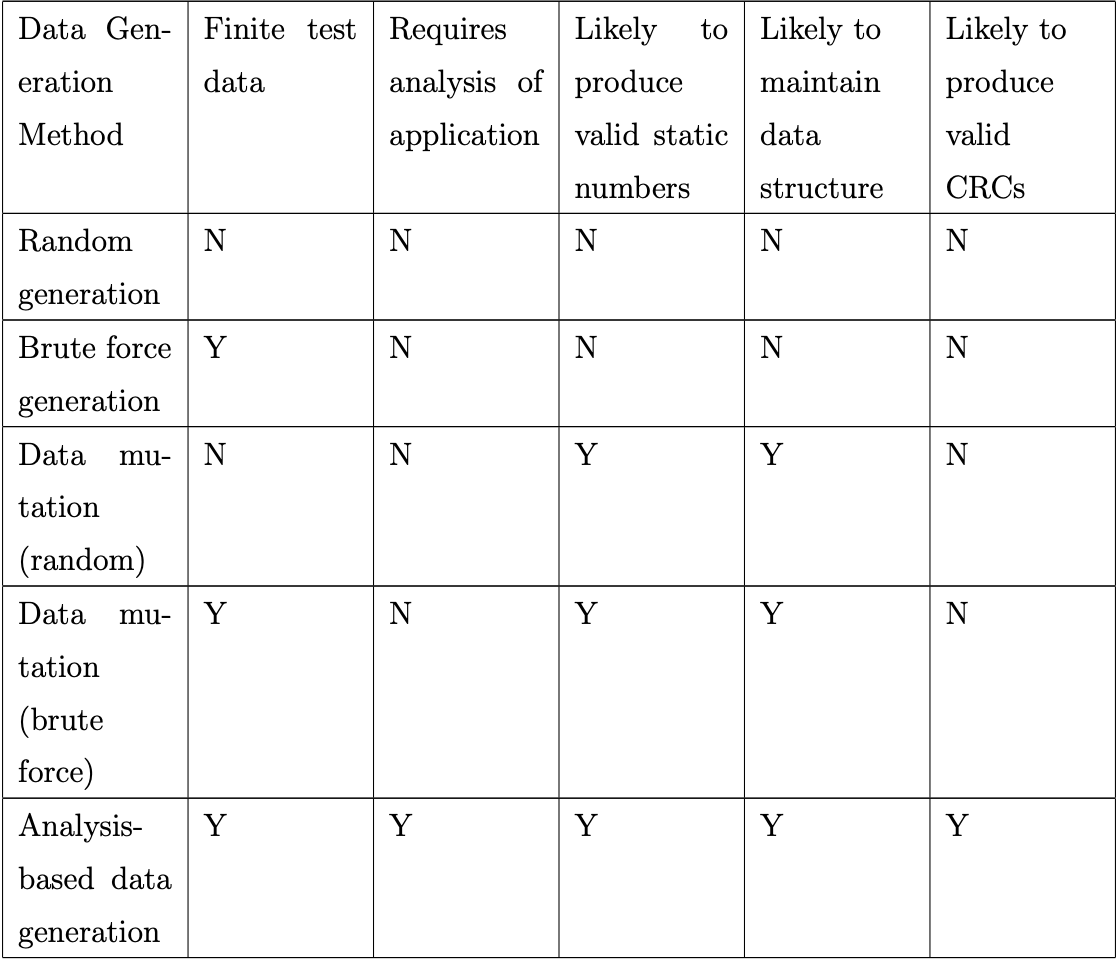
\includegraphics[width=0.489\textwidth]{Sources/testdata}
		\caption{Comparison of test data generation approaches}
		\label{fig:testdata}
	\end{figure}
	
	%Fuzzy Testing vs Other Fuzzy Testing techniques
	%Explain the context of these comparisons
	\subsection{Smart Fuzzing and Dumb Fuzzing}
		`Dumb Fuzzing' is the mutation of existing inputs that were initially valid \cite{defcon4}. Test cases in dumb fuzzing should be similar to normal program inputs but contain anomalies that defy the programmer's assumptions and reveal bugs \cite{defcon4}. These anomalies and mutations include modifying bytes or adding invalid characters, and do not require program or protocol knowledge. `Smart Fuzzing', also known as Generational Fuzzing, is the generation of test data using the protocol description, but it takes a long time to create the test inputs and requires complete knowledge of the program and/or protocol \cite{defcon4}. Charles Miller compared the code coverage of Smart Fuzzers and Dumb Fuzzers and found that Generational Fuzzing executed between two and five times more code than Dumb Fuzzing \cite{defcon4}. Dumb Fuzzers had a wide variance of effectiveness in covering the code since "the right inputs" were able to double the code coverage once mutated.
	
	\subsection{Static Analysis}
		Jacob West presented an analysis of fuzzy testing and static analysis at the 2007 DEF CON hacker convention \cite{defcon5}. According to \cite{defcon5}, fuzzy testing worked much faster than Static Analysis, but missed critical bugs "within its reach" and would have missed "bugs behind complex conditions (bugs hidden behind multiple header conditions)" \cite{defcon5}. As compared to Static Analysis, fuzzy testing:
		\begin{itemize}
			\item{does not require understanding of code;}
			\item{does not require source code access, and;}
			\item{produce demonstrable exploits with minimal human effort.}
		\end{itemize}
		However, Static Analysis is more thorough and will catch more bugs, is easier to do because it does not require running the source code, and can find vulnerabilities hidden by in-code error-handling and error-processing \cite{defcon5}.

\section{\label{sec:conclude}Conclusion}
	%Is fuzzy testing better or worse than other methods of testing and for which cases is it better?
	This paper provided a background of Fuzzy Testing, provided many instances of its use, and made the case for more adoption of its techniques. Fuzzy Testing has a large variability in its development and operation, and can be applied to any software application that has user input. Fuzzy Testing is increasingly cited as a necessary and fundamental piece of software testing \cite{automation}. It is very quick to apply, especially when using purely random test data generation. More research needs to be done though, as there are not many research projects that compare fuzzy testing with other black- or white-box testing methods. While most effective when testing for security vulnerabilities, it should also be implemented to the development life cycle of every software project since it takes little effort and is completely automated.
	
%Appendices
%\appendices
%	\section{}
%		Stuffity stuff stuff stuff
%	\section{}
%		More stuffy things
	
%Bibliography
%\nocite{*} %to include not-cited bibliography entries
\newpage
\bibliographystyle{IEEEtran}
\bibliography{IEEEabrv,bibliography}

\end{document}
